\chapter{Memory management in NekPy}
\label{sec:nekpy:memory}

A significant amount of effort has been invested into developing efficient
memory management techniques, to enable the sharing of memory between Python and
C++ for the ubiquitous \nek{} \inltt{Array} structure which is used throughout
the code.  The computations carried out in \nek{} are usually highly demanding
on the machines they are run on, therefore any unnecessary data duplication or
memory leaks would be detrimental to software performance.

This section first outlines some precusor information relating to the basics of
memory management in C++ and Python, before explaining the strategy used in
NekPy to effectively use the resources when passing data between the different
layers of the bindings.

\section{Memory management in C++ and Python}

\subsection{C++}

In C++ the memory used by the application is divided into five containers \cite{C++Memory}:
\begin{itemize}
    \item text segment -- containing the set of instructions for the program to execute;
    \item data segment -- containing static and global variables initialised with values, 
    e.g. \texttt{float pi = 3.14;} -- the size of the data segment is pre-determined at 
    the time of the compilation of the program and depends on the size of the variables 
    in the source code;
    \item bss (block started by symbol) segment -- containing static and global variables 
    not explicitly initialised with any value, e.g. \texttt{int n;} -- the size of the 
    data segment is pre-determined at the time of the compilation of the program and 
    depends on the size of the variables in the source code;
    \item stack -- a LIFO (last in, first out) structure containing the function calls 
    and variables intialised in the functions -- the size of the stack is pre-determined 
    at the time of compilation of the program and depends on the operating system and 
    development environment;
    \item heap -- containing all dynamically allocated memory (e.g. using instruction 
    \texttt{new} in C++).
\end{itemize}

The access to data on the heap is maintained by pointers which store the memory address of 
said data. If the pointer ceases to exist (e.g. because the function which contained it 
finished running and hence was taken off the stack) the programmer has no way of referencing 
the data on the heap again. The unused, inaccessible data will stay in the memory, consuming 
valuable resources if not properly deallocated using \texttt{delete} instruction. Issues may 
arise if the same memory address is held by two different pointers -- the deallocation of 
memory can render one of the pointers empty and possibly lead to errors.

In order to facilitate memory management, C++11 standard introduced shared pointers 
(\texttt{shared\_ptr})~\cite{C++SharedPtr}. Shared pointers maintain a reference counter 
which is increased when another shared pointer refers to the same memory address. The memory 
will only be deallocated when all shared pointers referencing the memory are destroyed, as shown 
in Figure~\ref{fig:shared_ptr}.

\begin{figure}[h!]
    \centering
    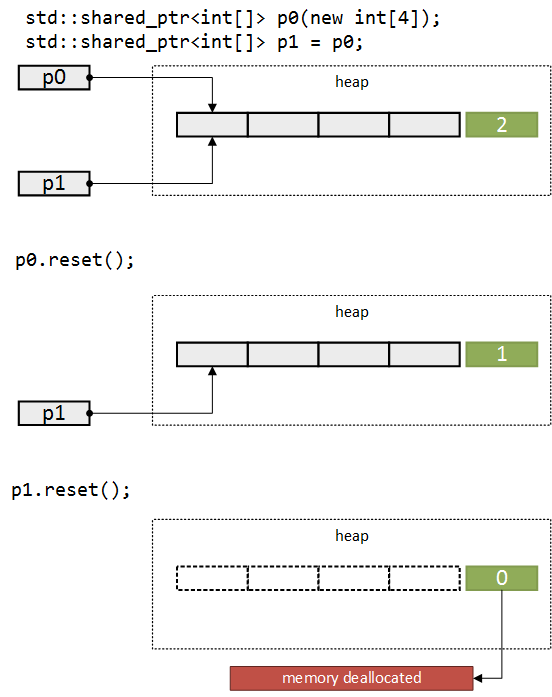
\includegraphics[width=0.6\textwidth]{img/shared_ptr}
    \caption{Memory management with C++11 \texttt{shared\_ptr}. The two declared shared pointers 
    reference an array of 4 integers. Reference counter shown in green.}
    \label{fig:shared_ptr}
\end{figure}

\subsubsection{Python}

Python manages memory though a private heap containing all Python objects~\cite{PythonMemory}. 
An internal memory manager is used to ensure the memory is properly allocated and deallocated 
while the script runs. In contrast to C++, Python's memory manager tries to optimise the memory 
usage as much as possible. For example, the same object reference is allocated to a new variable 
if the object already exists in memory. Another important feature of Python's memory manager is 
the use of garbage collector based on reference counting. When the object is no longer referenced 
by any variable the reference counter is set to zero, which triggers the garbage collector to free
the memory (possibly at some later time). A disadvantage of this solution is slower execution time,
since the garbage collector routines have to be called periodically. Features of the Python memory
manager are schematically shown in~Figure~\ref{fig:python_gc}

\begin{figure}[h!]
    \centering
    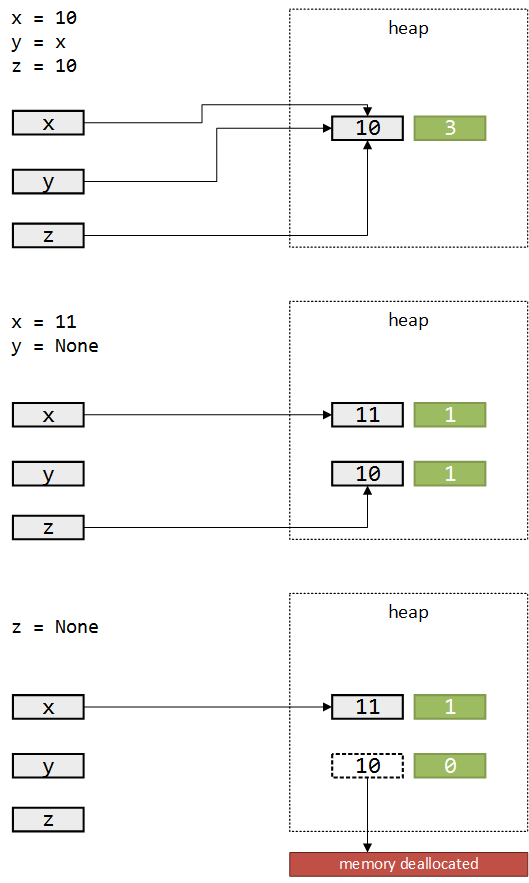
\includegraphics[width=0.6\textwidth]{img/python_gc}
    \caption{Memory management in Python. Memory is optimised as much as possible and garbage 
    collector deallocates the memory if the reference counter (shown in green) reaches 0.}
    \label{fig:python_gc}
\end{figure}

It is unusual for the Python programmer to manually modify the way Python uses
memory resources -- however it is sometimes necessary, as is the case with this
project. In particular, the Python C API exposes several macros to handle
reference counting, and developers can increase or decrease the reference
counter of the object using \texttt{Py\_INCREF} and \texttt{Py\_DECREF}
respectively~\cite{PythonManualMemory}. In \texttt{Boost.Python}, these calls
are wrapped in the \texttt{py::incref} and \texttt{py::decref} functions.

\section{Passing C++ memory to Python}

To highlight the technique for passing C++ memory natively into Python's
\texttt{ndarray}, we consider first the case of the native \nek{} matrix
structure. In many situations, matrices created by \nek{} (usually a
\texttt{shared\_ptr} of \texttt{NekMatrix<D, StandardMatrixTag>} type) need to
be passed to Python - for instance, when performing differentiation using
e.g. Gauss quadrature rules a differentiation matrix must be obtained. In order
to keep the program memory efficient, the data should not be copied into a NumPy
array but rather be referenced by the Python interface. This, however,
complicates the issue of memory management.

Consider a situation where C++ program no longer needs to work with the
generated array and the memory dedicated to it is deallocated. If this memory
has already been shares with Python, the Python interface may still require the
data contained within the array. However since the memory has already been
deallocated from the C++ side, this will typically cause an out-of-bounds memory
exception. To prevent such situations a solution employing reference counting
must be used.

\subsubsection{Converter method}

Boost.Python provides the methods to convert a C++ type element to one recognised by 
Python as well as to maintain appropriate reference counting. Listing \ref{lst:c_to_python} 
shows an abridged version of the converter method (for Python 2 only) with comments on 
individual parameters. The object requiring conversion is a \texttt{shared\_ptr} of 
\texttt{NekMatrix<D, StandardMatrixTag>} type (named \texttt{mat}).

\begin{lstlisting}[caption={Converter method for converting the C++ arrays into Python NumPy arrays.}, label={lst:c_to_python}, language=C++]
#include <LibUtilities/LinearAlgebra/NekMatrix.hpp>
#include <LibUtilities/LinearAlgebra/MatrixStorageType.h>
#include <NekPyConfig.hpp>

using namespace Nektar;
using namespace Nektar::LibUtilities;

template<typename T, typename F>
void NekMatrixCapsuleDestructor(void *ptr)
{
    // Destructor for shared_ptr when the capsule is deallocated.
    std::shared_ptr<NekMatrix<T, F>> *mat =
        (std::shared_ptr<NekMatrix<T, F>> *)ptr;
    delete mat;
}

template<typename T>
struct NekMatrixToPython
{
    static PyObject *convert(
        std::shared_ptr<NekMatrix<T, StandardMatrixTag>> const &mat)
    {
        // Create a PyCObject, which will hold a shared_ptr to the matrix.
        // When capsule is deallocated on the Python side, it will call the
        // destructor function above and release the shared_ptr reference.
        py::object capsule(py::handle<>(PyCObject_FromVoidPtr(
            new std::shared_ptr<NekMatrix<T, StandardMatrixTag>>(mat),
            NekMatrixCapsuleDestructor<T, StandardMatrixTag>)));

        int nRows = mat->GetRows(), nCols = mat->GetColumns();

        // increments Python reference counter to avoid immediate deallocation
        return py::incref( 
            np::from_data(
                mat->GetRawPtr(), // pointer to data
                np::dtype::get_builtin<T>(), // data type
                py::make_tuple(nRows, nCols), // shape of the array
                py::make_tuple(sizeof(T), nRows * sizeof(T)), // stride of the array
                capsule).ptr()); // capsule - contains the object owning the data (preventing it from being prematurely deallocated)
    }
}

template<typename T>
void export_NekMatrix()
{
    py::to_python_converter<std::shared_ptr<NekMatrix<T, StandardMatrixTag>>,
                            NekMatrixToPython<T>>();
}  
\end{lstlisting}

Firstly we give a brief overview of the general process undertaken during type
conversion. Boost.Python maintains a registry of known C++ to Python conversion
types, which by default allows for fundamental data type conversions such as
\texttt{double} and \texttt{float}. In this manner, many C++ functions can be
automatically converted, for example when they are used in \inltt{.def} calls
when registering a Python class. Clearly the \inltt{convert} function here
contains much of the functionality. In order to perform automatic conversion
between the \texttt{NekMatrix} and a 2D \texttt{ndarray}, we register the
conversion function inside Boost.Python's registry so that it is aware of the
datatypes. We also note that throughout the conversion code (and elsewhere in
NekPy), we make use of the Boost.NumPy bindings. These are a lightweight wrapper
around the NumPy C API, which simplifies the syntax somewhat and avoids direct
use of the API.

In terms of the conversion function itself, we first create a new Python capsule
object. The capsule is designed to hold a C pointer and a callback function that
is called when the Python object is deallocated. Since there is no Boost.Python
wrapper around this, we use a \texttt{handle<>} to wrap it in a generic
Boost.Python object. The strategy we therefore employ is to create a
\texttt{shared\_ptr}, which increases the reference counter of the
\texttt{NekMatrix}. This will prevent it being destroyed if it is in use in
Python, even if on the C++ side the memory is deallocated. The callback function
simply deletes the \texttt{shared\_ptr} when it is no longer required, cleaning
up the memory appropriately. This process is shown in
Figure~\ref{fig:c_to_python}. It is worth noting that the steps (c) and (d) can
be reversed and the \texttt{shared\_ptr} created by the Python binding can be
removed first.  In this case the memory will be deallocated only when the
\texttt{shared\_ptr} created by C++ is also removed.

\begin{figure}[h!]
    \centering
    \begin{subfigure}{0.6\textwidth}
        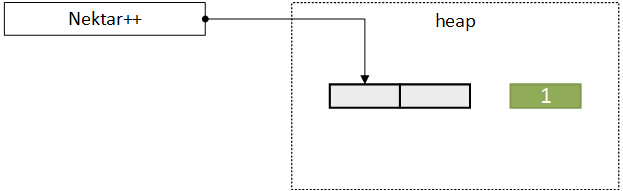
\includegraphics[width=0.99\textwidth]{img/c_to_python_a}
        \caption{Nektar++ creates a data array referenced by a \texttt{shared\_ptr}}
        \label{fig:c_to_python_a}
    \end{subfigure}
    \begin{subfigure}{0.6\textwidth}
        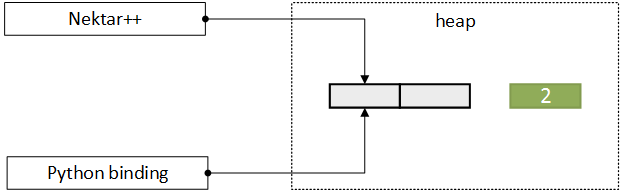
\includegraphics[width=0.99\textwidth]{img/c_to_python_b}
        \caption{Array is passed to Python binding which creates a new \texttt{shared\_ptr} 
        to the data}
        \label{fig:c_to_python_b}
    \end{subfigure}
    \begin{subfigure}{0.6\textwidth}
        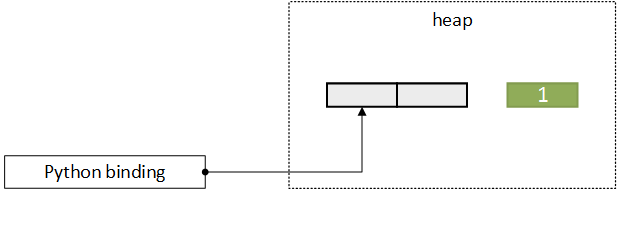
\includegraphics[width=0.99\textwidth]{img/c_to_python_c}
        \caption{Nektar++ no longer needs the data - its \texttt{shared\_ptr} is removed but 
        the memory is not deallocated}
        \label{fig:c_to_python_c}
    \end{subfigure}
    \begin{subfigure}{0.6\textwidth}
        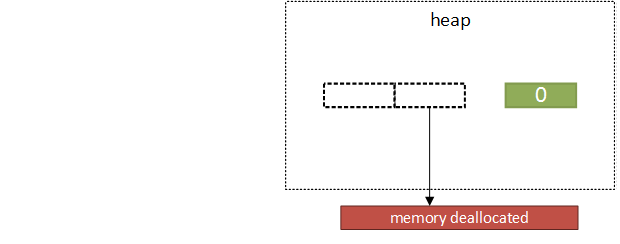
\includegraphics[width=0.99\textwidth]{img/c_to_python_d}
        \caption{When the data is no longer needed in the Python interface the destructor is 
        called and \texttt{shared\_ptr} is removed.}
        \label{fig:c_to_python_d}
    \end{subfigure}
    \caption{Memory management of data created in C++ using \texttt{shared\_ptr} and passed 
    to Python. Reference counter shown in green.}
    \label{fig:c_to_python}
\end{figure}

Finally, the converter method returns a NumPy array using the
\texttt{np::from\_data} method. Note that the \texttt{capsule} object is passed
as the \texttt{ndarray} base argument -- i.e. the object that owns the data. In
this case, when all \texttt{ndarray} objects that refer to the data become
deallocated, NumPy will not directly deallocate the data but instead release its
reference to the capsule. The capsule will then be deallocated, which will
decrement the counter in the \texttt{shared\_ptr}. We also note that data
ordering is important for matrix storage; \nek{} stores data in column-major
order, whereas NumPy arrays are traditionally row-major.  The stride of the
array has to be passed into the \texttt{np::from\_data} in a form of a tuple
\texttt{(a, b)}, where \texttt{a} is the number of bytes needed to skip to get
to the same position in the next row and \texttt{b} is the number of bytes
needed to skip to get to the same position in the next column. In order to stop
Python from immediately destroying the resulting NumPy array, its reference
counter is manually increased before the array is passed on to Boost.Python and
eventually returned to the user's code.

\subsubsection{Testing}

The process outlined above requires little manual intervention from the
programmer. There are no almost no explicit calls to Python C API (aside from
creating a \texttt{PyObject} -- \texttt{PyCObject\_FromVoidPtr}) as all
operations are carried out by Boost.Python. Therefore, the testing focused
mostly on correctness of returned data, in particular the order of the array. To
this end, the \emph{Differentiation} tutorials were used as tests. In order to
correctly run the tutorials the Python wrapper needs to retrieve the
differentiation matrix which, as mentioned before, has to be converted to a
datatype Python recognises. The test runs the differentiation tutorials and
compares the final result to the fixed expected value. The test is automatically
run as a part of \texttt{ctest} command if both the Python wrapper and the
tutorials have been built.

\subsection{Passing Python data to C++} 

Conversely, a similar problem exists when data is created in Python and has to
be passed to the C++ program. In this case, as the data is managed by Python,
the main reference counter should be maintained by the Python object and
incremented or decremented as appropriate using \texttt{py::incref} and
\texttt{py::decref} methods respectively. Although we do not support this
process for the \texttt{NekMatrix} as described above, we do use this process
for the \texttt{Array<OneD, >} structure. When the array is no longer needed by
the C++ program the reference counter on the Python side should be decremented
in order for Python garbage collection to work appropriately -- however this
should only happen when the array was created by Python in the first place.

The files implementing the below procedure are:

\begin{itemize}
  \item \texttt{LibUtilities/Python/BasicUtils/SharedArray.cpp} and
  \item \texttt{LibUtilities/BasicUtils/SharedArray.hpp}
\end{itemize}

\subsubsection{Modifications to \texttt{Array<OneD, const DataType>} class template}

In order to perform the operations described above, the C++ array structure
should contain information on whether or not it was created from data managed by
Python. To this end, two new attributes were added to C++ \texttt{Array<OneD,
  const DataType>} class template in the form of a \texttt{struct}:

\begin{lstlisting}[language=C++]
struct PythonInfo {
    void *m_pyObject; // Underlying PyObject pointer
    void (*m_callback)(void *); // Callback
};
\end{lstlisting}

where:

\begin{itemize}
  \item \texttt{m\_pyObject} is a pointer to the \texttt{PyObject} containing
  the data, which should be an \texttt{ndarray};
  \item \texttt{m\_callback} is a function pointer to the callback function
  which will decrement the reference counter of the \texttt{PyObject}.
\end{itemize}

Inside \texttt{Array<OneD, >}, this struct is held as a double pointer, i.e.:
\begin{lstlisting}[language=C++]
PythonInfo **m_pythonInfo;
\end{lstlisting}
This is done because if the \texttt{ndarray} was created originally from a C++
to Python conversion (as outlined in the previous section), we need to convert
the Array -- and any other shared arrays that hold the same C++ memory -- to
reference the Python array. If we did not do this, then it is possible that the
C++ array could be destroyed whilst it is still used on the Python side, leading
to an out-of-bounds exception. By storing this as a double pointer, in a similar
fashion to the underlying reference counter \texttt{m\_count}, we can ensure
that all C++ arrays are updated when necessary. We can keep track of Python
arrays by checking \texttt{*m\_pythonInfo}; if this is not set to
\texttt{nullptr} then the array has been constructed throught the Python to C++
converter.

Adding new attributes to the arrays might cause a significantly increased memory
usage or additional unforeseen overheads, although this was not seen in
benchmarking. However to avoid all possibility of this, a preprocessor directive
has been added to only include the additional arguments if \texttt{NekPy} had
been built (using the option \texttt{NEKTAR\_BUILD\_PYTHON}).

A new constructor has been added to the class template, as seen in Listing \ref{lst:new_const}. 
\texttt{m\_memory\_pointer} and \texttt{m\_python\_decrement} have been set to 
\texttt{nullptr} in the pre-existing constructors. A similar constructor was added for 
\texttt{const} arrays to ensure that these can also be passed between the languages. Note that 
no calls to Nektar++ array initialisation policies are made in this constructor, unlike in 
the pre-existing ones, as there is no need for the new array to copy the data.

\begin{lstlisting}[caption={New constructor for initialising arrays created through the Python to C++ converter method.}, label={lst:new_const}, language=C++]
Array(unsigned int dim1Size, DataType* data, void* memory_pointer, void (*python_decrement)(void *)) :
    m_size( dim1Size ),
    m_capacity( dim1Size ),
    m_data( data ),
    m_count( nullptr ),
    m_offset( 0 )                               
{
    m_count = new unsigned int(); 
    *m_count = 1;

    m_pythonInfo = new PythonInfo *();
    *m_pythonInfo = new PythonInfo();
    (*m_pythonInfo)->m_callback = python_decrement;
    (*m_pythonInfo)->m_pyObject = memory_pointer;
}
\end{lstlisting}

Changes have also been made to the destructor, as shown in Listing~\ref{lst:destructor}, 
in order to ensure that if the data was initially created in Python the callback function 
would decrement the reference counter of the NekPy array object. The detailed procedure 
for deleting arrays is described further in this section.

\begin{lstlisting}[caption={The modified destructor for C++ arrays.}, label={lst:destructor}, language=C++]
~Array()
{
    if( m_count == nullptr )
    {
        return;
    }

    *m_count -= 1;
    if( *m_count == 0 )
    {
        if (*m_pythonInfo == nullptr)
        {
            ArrayDestructionPolicy<DataType>::Destroy( m_data, m_capacity );
            MemoryManager<DataType>::RawDeallocate( m_data, m_capacity );
        }
        else
        {
            (*m_pythonInfo)->m_callback((*m_pythonInfo)->m_pyObject);
            delete *m_pythonInfo;
        }

        delete m_pythonInfo;
        delete m_count; // Clean up the memory used for the reference count.
    }
}
\end{lstlisting}

\subsubsection{Creation of new arrays}

The following algorithm has been proposed to create new arrays in Python and allow the 
C++ code to access their contents:

\begin{enumerate}
  \item The NumPy array object to be converted is passed as an argument to a C++
  method available in the Python wrapper.
  \item The converter method is called to convert a Python NumPy array into C++
  \texttt{Array<OneD, const DataType>} object.
  \item If the NumPy array was created through the C++-to-Python process (which
  can be determined by checking the \texttt{base} of the NumPy array), then:
  \begin{itemize}
    \item extract the \nek{} Array from the capsule;
    \item convert the Array (and all of its other references) to a Python array
    so that any C++ arrays that share this memory also know to call the
    appropriate decrement function;
    \item set the NumPy array's \texttt{base} to an empty object to destroy the
    original capsule.
  \end{itemize}
  \item Otherwise, the converter creates a new \texttt{Array<OneD, const DataType>} object
  with the following attribute values:
  \begin{itemize}
    \item \texttt{data} points to the data contained by the NumPy array,
    \item \texttt{memory\_pointer} points to the NumPy array object,
    \item \texttt{python\_decrement} points to the function decrementing the
    reference counter of the \texttt{PyObject},
    \item subsequently, \texttt{m\_count} is equal to 1.
  \end{itemize}
  \item The Python reference counter of the NumPy array object is increased.
  \item If any new references to the array are created in C++ the
  \texttt{m\_count} attribute is increased accordingly. Likewise, if new
  references to NumPy array object are made in Python the reference counter
  increases.
\end{enumerate}

The process is schematically shown in Figure \ref{fig:array_creation_deletion_a} 
and \ref{fig:array_creation_deletion_b}.

\subsubsection{Array deletion}

The array deletion process relies on decrementing two reference counters: one 
on the Python side of the program (Python reference counter) and the other one 
on C++ side of the program. The former registers how many Python references to 
the data there are and if there is a C++ reference to the array. The latter 
(represented by \texttt{m\_count} attribute) counts only the number of references 
on the C++ side and as soon as it reaches zero the callback function is triggered to 
decrement the Python reference counter so that registers that the data is no longer 
referred to in C++. Figure \ref{fig:array_deletion} presents the overview of the 
procedure used to delete the data.

In short, the fact that C++ uses the array is represented to Python as just an 
increment to the object reference counter. Even if the Python object goes out 
of scope or is explicitly deleted, the reference counter will always be non-zero 
until the callback function to decrement it is executed, as shown in Figure 
\ref{fig:array_creation_deletion_c}. Similarly, if the C++ array is deleted first, 
the Python object will still exist as the reference counter will be non-zero 
(see Figure \ref{fig:array_creation_deletion_d}).

\subsubsection{Converter method}

As with conversion from C++ to Python, a converter method was registered to make
Python NumPy arrays available in C++ with Boost.Python, which can be found in
the \texttt{SharedArray.cpp} bindings file.  In essence, Boost.Python provides
the used with a memory segment (all expressions containing
\texttt{rvalue\_from\_python} are to do with doing that). The data has to be
extracted from PyObject in order to be presented in a format C++ knows how to
read -- the \texttt{get\_data} method allows the programmer to do it for NumPy
arrays. Finally, care must be taken to manage memory correctly, thus the use of
borrowed references when creating Boost.Python object and the incrementation of
PyObject reference counter at the end of the method.

The callback decrement method is shown below in Listing \ref{lst:callback}. 
When provided with a pointer to PyObject it decrements it reference counter.

\begin{lstlisting}[caption={The decrement method called when the \texttt{m\_count} of C++ array reaches 0.}, label={lst:callback}, language=C++]
static void decrement(void *objPtr) 
    {
        PyObject *pyObjPtr = (PyObject *)objPtr;
        Py_XDECREF(pyObjPtr);
    }
\end{lstlisting}

\begin{figure}[h!]
    \centering
    \begin{subfigure}{0.9\textwidth}
        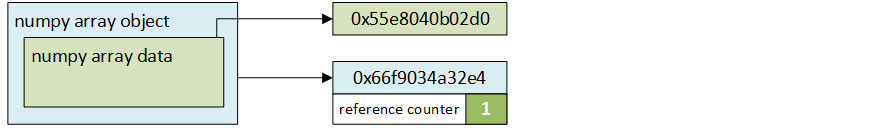
\includegraphics[width=0.99\textwidth]{img/array_creation_deletion_a}
        \caption{The NumPy array is created in Python. Note that the NumPy 
        object and the data it contains are represented by two separate memory addresses.}
        \label{fig:array_creation_deletion_a}
    \end{subfigure}
    \begin{subfigure}{0.9\textwidth}
        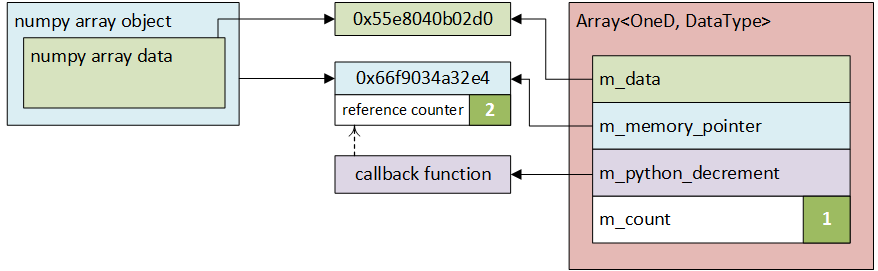
\includegraphics[width=0.99\textwidth]{img/array_creation_deletion_b}
        \caption{The C++ array is created through the converter method: its attributes 
        point to the appropriate memory addresses and the reference counter of the 
        memory address of NumPy array object is incremented.}
        \label{fig:array_creation_deletion_b}
    \end{subfigure}
    \begin{subfigure}{0.9\textwidth}
        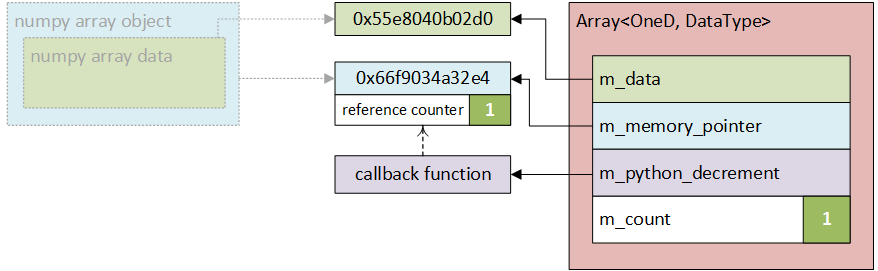
\includegraphics[width=0.99\textwidth]{img/array_creation_deletion_c}
        \caption{If the NumPy object is deleted first, the reference counter is 
        decremented, but the data still exists in memory.}
        \label{fig:array_creation_deletion_c}
    \end{subfigure}
    \begin{subfigure}{0.9\textwidth}
        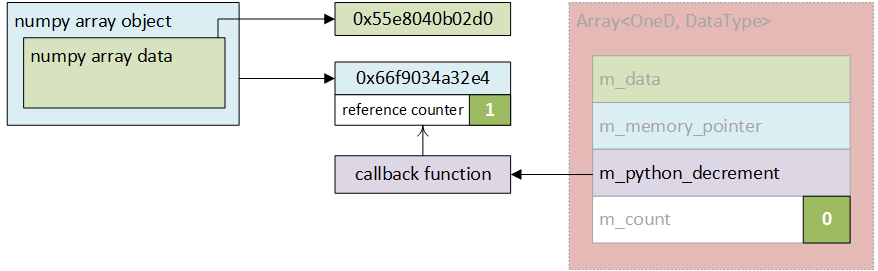
\includegraphics[width=0.99\textwidth]{img/array_creation_deletion_d}
        \caption{If the C++ array is deleted first, the callback function decrements 
        the reference counter of the NumPy object but the data still exists in memory.}
        \label{fig:array_creation_deletion_d}
    \end{subfigure}
    \caption{Diagram showing the process of creation and deletion of arrays. Reference 
    counters shown in green.}
    \label{fig:array_creation_deletion}
\end{figure}

\clearpage

\begin{figure}[h!]
    \centering
    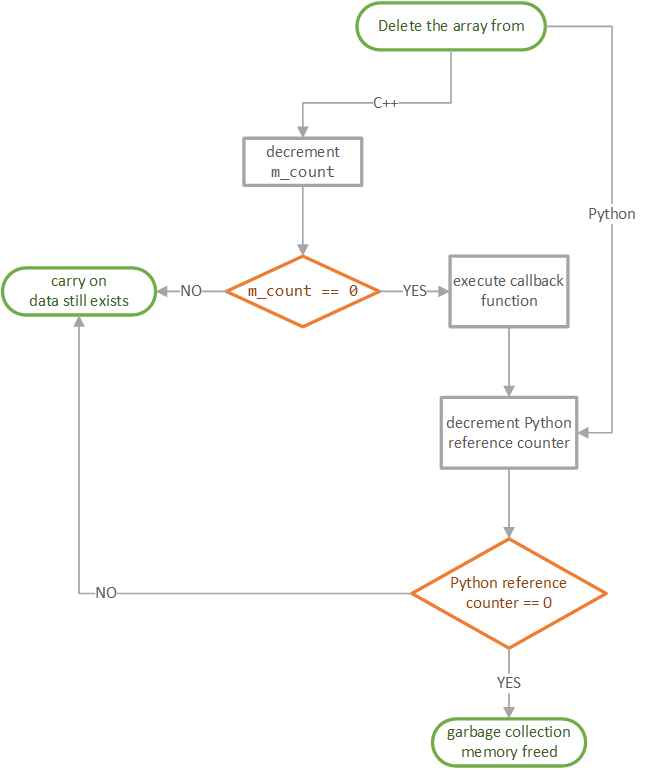
\includegraphics{img/deletion_flowchart}
    \caption{Flowchart describing the procedure for array deletion from either side of 
    the code.}
    \label{fig:array_deletion}
\end{figure}

\subsubsection{Testing}

As the process of converting arrays from Python to C++ required making direct calls to 
C API and relying on custom-written methods, more detailed testing was deemed necessary. 
In order to thoroughly check if the conversion works as expected, three tests were 
conducted to determine whether the array is:

\begin{enumerate}
\item referenced (not copied) between the C++ program and the Python wrapper,
\item accessible to C++ program after being deleted in Python code,
\item accessible in Python script after being deleted from C++ objects.
\end{enumerate}

Python files containing test scripts are currently located in 
\path{library\Demos\Python\tests}. They should be converted into unit tests 
that should be run when Python components are built.
